\documentclass{beamer}
\mode<presentation>
\usepackage{amsmath}
\usepackage{amssymb}
%\usepackage{advdate}
%\usepackage{gvv}
%\usepackage{gvv-book}
\usepackage{graphicx}
\usepackage{adjustbox}
\usepackage{subcaption}
\usepackage{enumitem}
\usepackage{multicol}
\usepackage{mathtools}
\usepackage{listings}
\usepackage{url}
\def\UrlBreaks{\do\/\do-}
\usetheme{Boadilla}
\usecolortheme{lily}
\let\vec\mathbf
\newcommand{\myvec}[1]{\ensuremath{\begin{pmatrix}#1\end{pmatrix}}}
\setbeamertemplate{footline}
{
  \leavevmode%
  \hbox{%
  \begin{beamercolorbox}[wd=\paperwidth,ht=2.25ex,dp=1ex,right]{author in head/foot}%
    \insertframenumber{} / \inserttotalframenumber\hspace*{2ex} 
  \end{beamercolorbox}}%
  \vskip0pt%
}
\setbeamertemplate{navigation symbols}{}

\providecommand{\nCr}[2]{\,^{#1}C_{#2}} % nCr
\providecommand{\nPr}[2]{\,^{#1}P_{#2}} % nPr
\providecommand{\mbf}{\mathbf}
\providecommand{\pr}[1]{\ensuremath{\Pr\left(#1\right)}}
\providecommand{\qfunc}[1]{\ensuremath{Q\left(#1\right)}}
\providecommand{\sbrak}[1]{\ensuremath{{}\left[#1\right]}}
\providecommand{\lsbrak}[1]{\ensuremath{{}\left[#1\right.}}
\providecommand{\rsbrak}[1]{\ensuremath{{}\left.#1\right]}}
\providecommand{\brak}[1]{\ensuremath{\left(#1\right)}}
\providecommand{\lbrak}[1]{\ensuremath{\left(#1\right.}}
\providecommand{\rbrak}[1]{\ensuremath{\left.#1\right)}}
\providecommand{\cbrak}[1]{\ensuremath{\left\{#1\right\}}}
\providecommand{\lcbrak}[1]{\ensuremath{\left\{#1\right.}}
\providecommand{\rcbrak}[1]{\ensuremath{\left.#1\right\}}}
\theoremstyle{remark}
\newtheorem{rem}{Remark}
\newcommand{\sgn}{\mathop{\mathrm{sgn}}}
\providecommand{\abs}[1]{\vert#1\vert}
\providecommand{\res}[1]{\Res\displaylimits_{#1}} 
\providecommand{\norm}[1]{\lVert#1\rVert}
\providecommand{\mtx}[1]{\mathbf{#1}}
\providecommand{\mean}[1]{E[ #1 ]}
\providecommand{\fourier}{\overset{\mathcal{F}}{ \rightleftharpoons}}
%\providecommand{\hilbert}{\overset{\mathcal{H}}{ \rightleftharpoons}}
\providecommand{\system}[1]{\overset{\mathcal{#1}}{ \longleftrightarrow}}
%\providecommand{\system}{\overset{\mathcal{H}}{ \longleftrightarrow}}
	%\newcommand{\solution}[2]{\vec{Solution:}{#1}}
%\newcommand{\solution}{\noindent \vec{Solution: }}
\providecommand{\dec}[2]{\ensuremath{\overset{#1}{\underset{#2}{\gtrless}}}}



\lstset{
%language=C,
frame=single, 
breaklines=true,
columns=fullflexible
}
\lstset{
  language=C,
  basicstyle=\ttfamily\footnotesize,
  keywordstyle=\color{blue}\bfseries,
  commentstyle=\color{gray}\itshape,
  stringstyle=\color{orange},
  numbers=left,
  numberstyle=\tiny\color{gray},
  breaklines=true,
  frame=single,
  showstringspaces=false,
  tabsize=4,
  captionpos=b
}
\numberwithin{equation}{section}
\lstset{
  language=Python,
  basicstyle=\ttfamily\small,
  keywordstyle=\color{blue},
  stringstyle=\color{orange},
  numbers=left,
  numberstyle=\tiny\color{gray},
  breaklines=true,
  showstringspaces=false
}

\title{Problem 1.4.5}
\author{Sujal Rajani}

\date{\today} 
\begin{document}

\begin{frame}
\titlepage
\end{frame}



\begin{frame}{Question}
\textbf{Question}:


\noindent Find the coordinates of the point $\vec{P}$ on AD such that AP : PD = 2 : 1.    
\end{frame}

\begin{frame}{Solution}
\textbf{Solution:} 

As nothing is mentioned in the question about the coordinates of A and D , so we are assuming the coordinates of A as (2,2) ,D as (-1,-1) .
\begin{align}
			\vec A = \myvec{2\\2},\vec D = \myvec{-1\\-1}.
\end{align}
as mentioned in the question $\vec{P}$ is dividing the join of A and D in $2:1$.

so for finding the position vector of $\vec{P}$ we are using section formula 
\end{frame} 

\begin{frame}{section formula }
    \textbf{section formula }

If $\vec{D}$ divides BC in the ratio k : 1
\begin{align*}
     \vec{D}=\dfrac{k\vec{C}+\vec{B}}{k+1}
\end{align*}

\end{frame}
\begin{frame}{OBTAINING COORDINATES}
\\
\quad k=2
\\

    the position vector of $\vec{P}$ is : 
\begin{align*}
     \vec{P}=\dfrac{2\vec{D}+\vec{A}}{2+1}
     \\
     \vec{P}=\dfrac{2\myvec{-1\\-1}+\myvec{2\\2}}{2+1}=\myvec{0\\0}
\end{align*}

\end{frame}

    
       \begin{frame}[fragile]
    \begin{figure}[H]
    \centering
    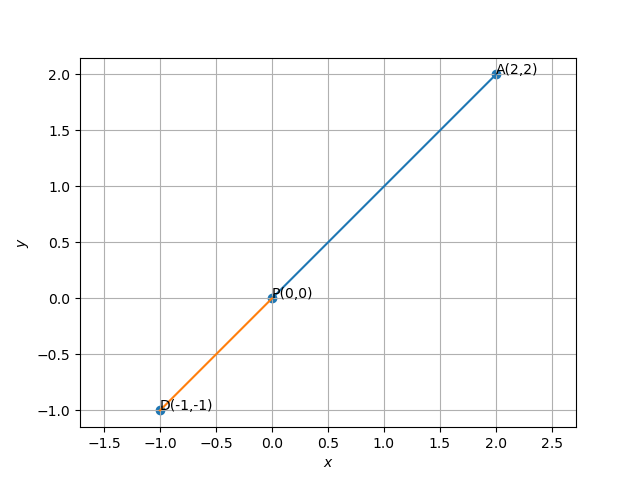
\includegraphics[width = 0.6\columnwidth]{../figs/img.png}
    \caption*{}
    \label{figs}
\end{figure}
\end{frame}
\section{ C Code}
\begin{frame}[fragile]
\frametitle{C Code }
\begin{lstlisting}[language=C]
#include <stdio.h>

int main() {
    // Coordinates of A and D
    float Ax = 2.0, Ay = 2.0;
    float Dx = -1.0, Dy = -1.0;

    // Ratio AP:PD = 2:1
    float m = 2.0, n = 1.0;

    // Section formula: P = (m*D + n*A)/(m+n)
    float Px = (m*Dx + n*Ax) / (m + n);
    float Py = (m*Dy + n*Ay) / (m + n);

    printf("The coordinates of point P are: (%.2f, %.2f)\n", Px, Py);
    return 0;
}
    
\end{lstlisting}
\end{frame}



\begin{frame}[fragile]
\frametitle{Python Code for Plotting}
\begin{lstlisting}[language=Python]
import math
import sys   

import numpy as np
import numpy.linalg as LA
import matplotlib.pyplot as plt
import matplotlib.image as mpimg
from line.funcs import *
#from triangle.funcs import *
#from conics.funcs import circ_gen
#if using termux
import subprocess
import shlex
#end if

A = np.array([2,2]).reshape(-1,1)
P = np.array([0,0]).reshape(-1,1)
D = np.array([-1,-1]).reshape(-1,1)
coords = np.block([[A,P,D]])

\end{lstlisting}

\end{frame}
\section{Python Code}
\begin{frame}[fragile]
\frametitle{Python Code for Plotting}
\begin{lstlisting}[language=Python]   

AP = line_gen(A,P)
PD = line_gen(P,D)

plt.plot(AP[0,:],AP[1,:])
plt.plot(PD[0,:],PD[1,:])

plt.scatter(coords[0,:],coords[1,:])


plt.text(A[0],A[1],"A(2,2)")
plt.text(P[0],P[1],"P(0,0)")
plt.text(D[0],D[1],"D(-1,-1)")


\end{lstlisting}

\end{frame}
\begin{frame}[fragile]
\frametitle{Python Code for Plotting}
\begin{lstlisting}[language=Python]   

plt.xlabel('$x$')
plt.ylabel('$y$')
plt.legend(loc='best')
plt.grid() # minor
plt.axis('equal')

plt.savefig('../figs/img.png')



\end{lstlisting}

\end{frame}
\end{document}